% Template for Cogsci submission with R Markdown

% Stuff changed from original Markdown PLOS Template
\documentclass[10pt, letterpaper]{article}

\usepackage{cogsci}
\usepackage{pslatex}
\usepackage{float}
\usepackage{caption}

% amsmath package, useful for mathematical formulas
\usepackage{amsmath}

% amssymb package, useful for mathematical symbols
\usepackage{amssymb}

% hyperref package, useful for hyperlinks
\usepackage{hyperref}

% graphicx package, useful for including eps and pdf graphics
% include graphics with the command \includegraphics
\usepackage{graphicx}

% Sweave(-like)
\usepackage{fancyvrb}
\DefineVerbatimEnvironment{Sinput}{Verbatim}{fontshape=sl}
\DefineVerbatimEnvironment{Soutput}{Verbatim}{}
\DefineVerbatimEnvironment{Scode}{Verbatim}{fontshape=sl}
\newenvironment{Schunk}{}{}
\DefineVerbatimEnvironment{Code}{Verbatim}{}
\DefineVerbatimEnvironment{CodeInput}{Verbatim}{fontshape=sl}
\DefineVerbatimEnvironment{CodeOutput}{Verbatim}{}
\newenvironment{CodeChunk}{}{}

% cite package, to clean up citations in the main text. Do not remove.
\usepackage{apacite}

% KM added 1/4/18 to allow control of blind submission


\usepackage{color}

% Use doublespacing - comment out for single spacing
%\usepackage{setspace}
%\doublespacing


% % Text layout
% \topmargin 0.0cm
% \oddsidemargin 0.5cm
% \evensidemargin 0.5cm
% \textwidth 16cm
% \textheight 21cm

\title{Children's understanding of others' lexical knowledge}

\usepackage{booktabs}
\usepackage{longtable}
\usepackage{array}
\usepackage{multirow}
\usepackage{wrapfig}
\usepackage{float}
\usepackage{colortbl}
\usepackage{pdflscape}
\usepackage{tabu}
\usepackage{threeparttable}
\usepackage{threeparttablex}
\usepackage[normalem]{ulem}
\usepackage{makecell}
\usepackage{xcolor}



\newlength{\cslhangindent}
\setlength{\cslhangindent}{1.5em}
\newenvironment{CSLReferences}%
  {}%
  {\par}

\begin{document}

\maketitle

\begin{abstract}
To communicate successfully, you need to choose words that your partner
understands. Adults maintain precise models of the words people are
likely to know, using both their experience with their conversational
partner and general metalinguistic information. Do children also know
what words others unlike them are likely to know? We asked children ages
4-8 (\(n\) = 62) to predict whether a very young child would know each
of 15 familiar animal words, all typically acquired within a 6-month
range. With minimal information, even children as young as 4 made
reliable predictions about the target child's lexical knowledge.
Further, children's accuracies improved significantly over the course of
development, as did the sophistication of their explanations for their
judgments. Thus, even preschool age children have access to some
information that would let them tailor their speech to younger children
(such as siblings), and by the time they enter school, children may have
just as much information as adults.

\textbf{Keywords:}
communication, metalinguistic, knowledge reasoning, cognitive
development
\end{abstract}

\hypertarget{introduction}{%
\section{Introduction}\label{introduction}}

Imagine visiting the zoo with your friend and their 2-year-old. As you
walk by the peacocks, you hear your friend say, ``Do you see those blue
birds?'' Immediately, you know that your friend is talking to their
child and not you. If they were talking to you, saying ``peacock'' would
be perfectly clear; however, ``blue bird'' might be a better description
for a child who has never seen a peacock before. Even when talking about
the same object, we use different words depending on what we think our
conversational partners know and don't know.

Adults track and adapt to their conversational partners' knowledge with
relative ease. For example, adults reduce the information they give when
re-telling a story to someone who has heard it before, but not when
telling the story to a new partner (Galati \& Brennan, 2010). Adults can
adapt even to partners who are quite different from them, as in the case
of parents and their children. Parents model the fine-grained details of
their children's vocabularies and use these models in spontaneous
communication (e.g.~using {``blue bird''} to describe a peacock, Leung,
Tunkel, \& Yurovsky, in press). These vocabulary models are shaped by
extensive individual parent-child interactions, but likely also general
metalinguistic knowledge--for instance, that shorter words are typically
simpler than longer words and thus learned earlier likely to be known.
In line with this conjecture, Kuperman, Stadthagen-Gonzalez, \&
Brysbaert (2012) asked people to report the age at which they understood
a set of 30,000 English words. They found that adults typically
overestimated the ages at which words are learned, but were quite
accurate at judging their relative order. Thus, even adults without
children have access to the kind of metalinguistic information they
could use to calibrate speech to children's knowledge.

Can children use this same kind of information to predict whether others
will know words? Pre-school age children are able to infer other
people's knowledge from relatively sparse information, such as age or
expertise (Jaswal \& Neely, 2006; Lutz \& Keil, 2002). Further, children
ascribe different levels of general knowledge to infants, preschool
children, and adults VanderBorght \& Jaswal (2009). However, reasoning
about another person's specific lexical knowledge may prove difficult
for young children. For instance, children often overattribute knowledge
to others, especially knowledge they themselves already have Ghrear,
Fung, Haddock, \& Birch (2020). Children as young as 5 have been shown
to make accurate metalinguistic judgments about their own vocabulary
knowledge (Walley \& Metsala, 1992). Can they use this knowledge to
reason about other children as well?

However, reasoning about another person's specific lexical knowledge may
prove difficult for young children as they also show consistent errors
in reasoning about other's knowledge, commonly over-attributing
knowledge Taylor, Esbensen, \& Bennett (1994). The bias to
over-attribute knowledge is particularly pronounced when the child
themselves knows the piece of information Ghrear, Fung, Haddock, \&
Birch (2020).

We ask how children infer another children's lexical knowledge, and
specifically whether they make word-level predictions in line with
expected AoA. Children at least as young as 5 can make metalinguistic
judgments about their own vocabulary knowledge, accurately estimating
the age and order in which they learned a variety of words (Walley \&
Metsala, 1992). In our study, we introduced 4- to 8-year-old children to
a younger fictional child, and asked them to make judgments about the
target child's knowledge of various familiar words. We find that even
4-year-olds make accurate inferences about the target child's knowledge,
and that older children's responses more closely correlate with adult
judgments of AoA.

We examined the development of children's use of metalinguistic lexical
knowledge, asking how children's abilities to make word-level knowledge
judgments about a younger child change over the preschool and early
school years. We found the accuracy of children's judgments improved
reliably from 4- to 8-years of age, bu that even the younger children's
judgments showed significant knowledge about the words that a younger
child was likely to know. Further, 7- and 8-year-old children were more
accurate than a comparison group of adults. {[}SOMETHING ABOUT
EXPLANATIONS{]}. These results suggest blah blah blah. {[}one sentence
about importance{]}.

\hypertarget{method}{%
\section{Method}\label{method}}

\hypertarget{stimuli}{%
\subsubsection{Stimuli}\label{stimuli}}

Our stimuli consisted of 15 words drawn from a single domain (animal
words), along with corresponding images of each animal. We pulled all
animal images (\(n\) = 45) from a normed image set Snodgrass \&
Vanderwart (1980). To ensure our stimuli set spanned a range of ages of
acquisition (AoAs), we ranked the animal words from earliest to latest
AoA, using data from Kuperman, Stadthagen-Gonzalez, \& Brysbaert (2012),
and split the words into five bins. In order to select animal images
that are recognizable and typically identified by a single name, we
chose the three animals from each AoA bin with the highest naming
agreement according to a naming task with children (Cycowicz, Friedman,
Rothstein, \& Snodgrass, 1997).

The resulting animals, order by AoA, were dog, duck, cat, pig, fish,
turtle, zebra, elephant, snake, penguin, gorilla, owl, raccoon, leopard,
and lobster. Although adult AoA estimates for these words range from 2.5
to 7.5 years old (Kuperman, Stadthagen-Gonzalez, \& Brysbaert, 2012),
all of these animal words are generally acquired by age 3 according to
parent reports of children's vocabulary knowledge (Frank, Braginsky,
Yurovsky, \& Marchman, 2017). Because the youngest children in our study
are 4 years old, we expected all participants to know these animal
words.

\textbf{add thing about why were using kuperman, expand on why it's an
okay thing to use, here or results}

\hypertarget{participants}{%
\subsubsection{Participants}\label{participants}}

We pre-registered a planned sample of 60 children ages 4-8, with 12
children recruited for each year-wise age group. Due to overrecruitment,
our final sample included 62 children (12 4-year-olds, 13 5-year-olds,
13 6-year-olds, 12 7-year-olds, 12 8-year-olds). All analyses hold when
looking only at the 60 children run first chronologically. Based on a
pre-registered exclusion criterion, children who failed to answer all of
the questions were excluded and replaced (an additional 7 children).
Families were recruited online, primarily through a US University
database of families who have expressed interest in doing research or
previously participated. Children completed this study over Zoom,
interacting with a live experimenter who navigated a slide-style,
animated Qualtrics survey.

A separate sample of 30 adults were recruited via Amazon Mechanical
Turk. The adult sample provides a simple test that our task elicits
robust inferences about the target child's lexical knowledge, and that
these inferences correspond to extant AoA data. Adult participants
completed the same task using Qualtrics, with minor modifications as
described below.

\hypertarget{procedure}{%
\subsection{Procedure}\label{procedure}}

\begin{CodeChunk}
\begin{figure}[tb]

{\centering 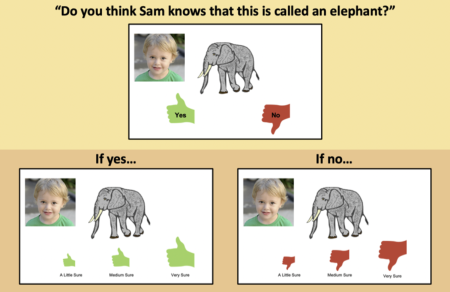
\includegraphics{figs/task-method-1} 

}

\caption[The structure of an example trial]{The structure of an example trial. The experimenter labeled the animal, then asks the child “Do you think Sam knows that this is called an elephant?” Based on their response, children were then asked to provide a confidence judgment on a 3-point scale (little sure, medium sure, very sure).}\label{fig:task-method}
\end{figure}
\end{CodeChunk}

\emph{Introduction.} Children were shown a picture of a child named
``Sam'' (seen in Figure \ref{fig:task-method}). Children were anchored
to Sam's knowledge of various familiar skills, specifically some skills
that Sam has acquired (e.g., coloring), and some that Sam has not yet
acquired (e.g., reading). Children were then specifically anchored to
Sam's possible word knowledge in an unrelated domain--given an example
of one word Sam knows (\emph{car}), and one word that Sam does npt know
(\emph{piano}). This introduction was intended to familiarize the
children with Sam, roughly anchor them to Sam's knowledge and age, and
to ensure that children understand there are things Sam does not know
yet (even things children themselves likely know, such as how to read).

\emph{Trial structure.} On each trial, children were shown a drawing of
a familiar object or animal (Rossion \& Pourtois, 2004). The
experimenter first labeled the object for the child (e.g., saying
``Look, it's {[}an elephant{]}!), and then asked the target child's
knowledge (e.g., saying,''Do you think Sam knows that this is called
{[}an elephant{]}? Yes or no?''). Based on their response, children were
then asked a follow-up question: ``How sure are you that Sam
{[}knows/doesn't know{]} that this is called {[}an elephant{]}--a little
sure, medium sure, or very sure?'' All questions were presented with
accompanying pictures of thumbs {[}up/down{]} of varying size (see
Figure \ref{fig:task-method}). Children as young as 3 are able to engage
in uncertainty monitoring and report confidence, although these skills
do develop in the preschool years (Lyons \& Ghetti, 2011). Children's
responses to these two items were recoded onto a 1-6 scale from
1--\emph{very sure Sam doesn't know} to 6--\emph{very sure Sam knows}.

The experimenter provided no evaluative feedback on any trials, but did
offer consistent neutral feedback (e.g., repeating the child's answer or
saying ``Okay!''). When a child failed to respond within about 5 seconds
or offered a non-canonical response (e.g., saying ``Maybe''), the
experimenter acknowledged the child's answer and then repeated the
question with the possible responses. If a child did not answer after
the question was repeated, the experimenter moved on and marked the
trial as no response. These were considered ``incomplete'' sessions and
these participants were not included in the final sample.

\emph{Familiarization trials.} Children first completed two non-animal
familiarization trials, one for an early-acquired word (ball) and one of
a late-acquired word (artichoke). These trials followed the trial
structure described above and were intended to help familiarize children
with the structure of the questions and scales. These trials were always
asked first and in a fixed order.

\emph{Animal trials.} Children were then shown 15 trials of the same
form (see example trial in Figure \ref{fig:task-method}). For the 15
animal trials, trial order was randomized across participants to control
for any potential order effects in children's responses.

\emph{Explanation.} After completing the final animal trial, children
were asked an open-ended explanation question about their final judgment
(e.g., ``Why do you think Sam {[}knows/doesn't know{]} that this is
called {[}an elephant{]}?''). Because the trial order was randomized,
the explanations concerned different animal words across participants.

\emph{Final check questions.} Children were asked two questions about
Sam's skill knowledge, one early acquired skill (going up and down
stairs) and one very late acquired skill (driving a car). These
questions again followed the general trial structure described above.
The skill knowledge items were included as an additional check that
children at all ages were able to use the scale appropriately, in case
young children failed to differentiate animal words based on AoA.
Lastly, children were asked to report how old they thought Sam was. This
question was intended to assess another aspect of children's belief
about Sam. Sam's photo and skill knowledge were intended to indicate
toddlerhood.

\hypertarget{adult-procedure.}{%
\paragraph{Adult procedure.}\label{adult-procedure.}}

Adult participants completed a minimally adapted version of the same
task online via Qualtrics. Unlike children, adults were simply presented
with the full 6-point scale (1--\emph{very sure Sam doesn't know} to
6--\emph{very sure Sam does know}). Additionally, the task was
administered asynchronously, so adult participants did not interact with
an experimenter or receive any feedback during the task. Otherwise, the
adult task was identical to the child task described above.

\begin{CodeChunk}
\begin{figure}[tb]
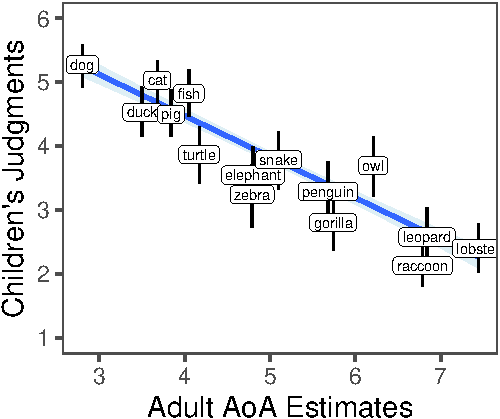
\includegraphics{figs/overall-1} \caption[Comparing adult AoA estimates (in years, taken from Kuperman et al., 2012) and children’s judgments on our 6-point scale (1 = very sure Sam doesn’t know]{Comparing adult AoA estimates (in years, taken from Kuperman et al., 2012) and children’s judgments on our 6-point scale (1 = very sure Sam doesn’t know; 6 = very sure Sam knows). The black lines show 95\% confidence intervals for each item. The shaded region shows one standard error based on a linear regression estimated from the raw data.}\label{fig:overall}
\end{figure}
\end{CodeChunk}

\hypertarget{results}{%
\section{Results}\label{results}}

Our primary analyses compare knowledge judgments on our 6-point scale to
AoA judgments from adults (taken from Kuperman, Stadthagen-Gonzalez, \&
Brysbaert, 2012). Data were analyzed using pre-registered mixed effects
model predicting children's judgments from adult AoA estimates
(Kuperman, Stadthagen-Gonzalez, \& Brysbaert, 2012), including random
effects for participant and word. Using the \texttt{lme4} package in
\texttt{R} (Bates, Mächler, Bolker, \& Walker, 2015). We our model
syntax was
\texttt{judgment\ \textasciitilde{}\ AoA\ +\ (1\ \textbar{}\ participant)\ +\ (1\ \textbar{}\ word)}.

We expected that overall, children's judgments would recover the ordinal
shape of age of acquisition data for these items. That is, children
would infer that the child is most likely to know early acquired words,
and least likely to know late acquired words. As a result, we expected a
negative relationship between judgments of the target child's lexical
knowledge and adult AoA estimates.

First, analyzing adults responses on our task, we saw the predicted
negative effect of AoA on adults' judgments of the target child's
knowledge (see Figure \ref{fig:development}, \(\beta =\) -0.63, \(t =\)
-8.71, \(p\) \textless{} .01). This confirms that our task is eliciting
reliable predictions from adults, and that adults' inferences about the
target child's knowledge match predictions from AoA estimation tasks
(Kuperman, Stadthagen-Gonzalez, \& Brysbaert, 2012).

\begin{CodeChunk}
\begin{figure*}[tb]
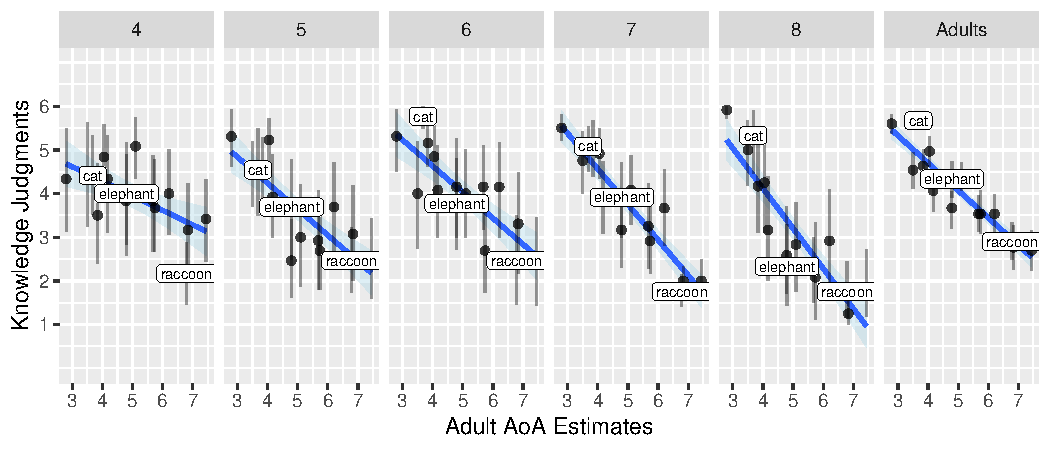
\includegraphics{figs/development-1} \caption[Children and adults judgements about the target child's word knowledge across development, compared with adult AoA estimates (in years, taken from Kuperman et al., 2012)]{Children and adults judgements about the target child's word knowledge across development, compared with adult AoA estimates (in years, taken from Kuperman et al., 2012). Each point represents 1 of the 15 word items, with black lines showing 95\% percent confidence intervals for each item. The shaded region shows one standard deviation based on a linear regression estimated from the raw data.}\label{fig:development}
\end{figure*}
\end{CodeChunk}

Do children's judgments about a child's vocabulary knowledge also
reflect a sensitivity to which words are learned later? To answer this
question looking at children's responses overall, we ran the model with
no age term and see a significant negative effect of AoA on children's
judgments (\(\beta =\) -0.65, \(t =\) -8.29, \(p\) \textless{} .001).
That is, overall, children judged that the target child would be most
likely to know an early acquired word (e.g., dog) and least likely to
know a late acquired word (e.g., lobster, see Figure \ref{fig:overall}).

We also expected developmental change in children's sensitivity to Sam's
vocabulary knowledge, with older children's judgments recovering
word-level AoA data more closely. To test for developmental changes in
children's responses, we used the same mixed effects model but included
an effect of age and an interaction between AoA and age. Our model
syntax was
\texttt{judgment\ \textasciitilde{}\ AoA\ *\ age\ +\ (1\ \textbar{}\ participant)\ +\ (1\textbar{}word)}.
We expected a significant interaction between AoA and child;s age,
consistent with older children/s judgments more closely reflecting
word-level AoA data. That is, when plotting children's judgments against
adult AoA estimates, older children would show steeper negative slopes
than younger children (Figure \ref{fig:development}). As above, our
model shows the same main effect of AoA that we saw in the overall model
(\(\beta =\) -0.65, \(t =\) -8.29, \(p\) \textless{} .001). We also see
a positive main effect of children's age on their ratings (\(\beta =\)
0.55, \(t =\) 3.68, \(p\) \textless{} .001). Crucially, we see the
expected interaction between child's age and adult's estimated AoA
(\(\beta =\) -0.14, \(t =\) -5.1, \(p\) \textless{} .001), suggesting
that children's judgments are becoming more adult-like in this age range
(Figure \ref{fig:development}).

\begin{CodeChunk}

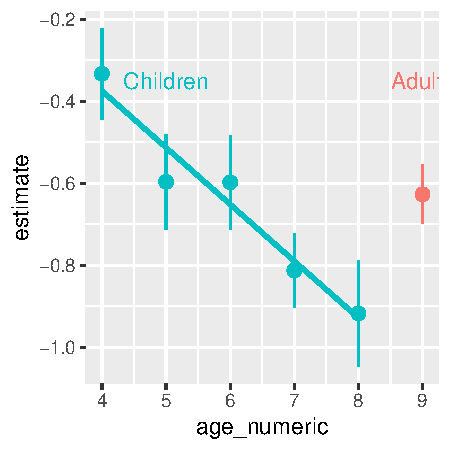
\includegraphics{figs/unnamed-chunk-6-1} \end{CodeChunk}

To test the robustness of this intuition at each age, we ran the above
model separately for each year-wise age group. While we see evidence of
developmental change above, this additional analysis helps us understand
if even young children are showing this intuition. We found a
significant negative effect of AoA on children'\,'\,'s judgments at all
age groups (with the smallest effect in 4-year-olds: \(\beta =\) -0.33,
\(t =\) -3.01, \(p =\) .01). That is, even 4-year-old children judged
that late-acquired animal words were less likely to be known by the
target child.

\hypertarget{secondary-results}{%
\subsection{Secondary Results}\label{secondary-results}}

\hypertarget{familiarization-trials.}{%
\paragraph{Familiarization trials.}\label{familiarization-trials.}}

Children completed two familiarization trials asking about the target
child's knowledge of two non-animal words (\emph{ball} and
\emph{artichoke}). These questions were primarily included to help
children get accustomed to the general trial structure. To analyze
children's responses on these familiarization items, we used a similar
mixed effects structure predicting children's knowledge judgments from
the item and a random effect of pariticpant.

Overall, children were significantly more likely to report that Sam
knows the word ``ball'' (\(mean =\) 4.65) than that Sam knows the word
``artichoke'' (\(mean =\) 1.87, \(\beta =\) 2.77, \(t =\) 10.6, \(p =\)
\textless{} .01). Analyzing judgments separately for each age group,
4-year-olds do not significantly differentiate the two familiarization
items (\(\beta =\) 0.17, \(t =\) 0.21, \(p =\) .83). All other age
groups signifcantly differentiated the two familiarization items
(\(ps <\) 0.05).

\hypertarget{skill-knowledge.}{%
\paragraph{Skill knowledge.}\label{skill-knowledge.}}

We included two questions about the target child's skill knowledge. In
the event that children at any age were differentiating the target
child's lexical knowledge, these questions were intended primarily as a
check that children at all ages were nevertheless able to use the scale
appropriately and able to infer knowledge in another domain. Note that
the two skill items (\emph{going up and down stairs}, and \emph{driving
a car}) are also in line with children's own knowledge, unlike the word
items. That is, child participants should be able to answer these
questions appropriately even if they are reasoning egocentrically about
their own knowledge.

Overall, children differentiated the target child's skill knowledge on
these two items. We used a similar mixed effects structure predicting
children's knowledge judgments from the item and a random effect of
pariticpant. Children were significantly more likely to report that the
child knows how to go up and down stairs (\(mean =\) 4.1) than that the
child knows how to drive a car (\(mean =\) 1.4, \(\beta =\) 2.69,
\(t =\) 10.29, \(p =\) \textless{} .01). Analyzing judgments separately
for each age group, even 4-year-olds were significantly differentiating
the two skill item (\(\beta =\) 2.33, \(t =\) 4.31, \(p =\) \textless{}
.01).

\hypertarget{explanations}{%
\subsubsection{Explanations}\label{explanations}}

\begin{table*}[tb]
\centering
\begin{tabular}{ll}
  \hline
Category & Example Utterance \\ 
  \hline
Language & Because it was a very long word. \\ 
    & Because it only has 3 letters. \\ 
  Experience & Because maybe he has a dog. \\ 
    & Because gorillas are really rare animals \\ 
  Location & Because penguins live in the artic and it's too cold for little kids... \\ 
    & Because fish swim under the ocean. \\ 
  Age & Because I think I knew that when I was around 3... \\ 
    & Because if he went to preschool then he probably knew it... \\ 
  Unsure & I don't know. \\ 
    & I'm not sure. \\ 
  Other & Because it had a longer beak than a bird. \\ 
    & Because it's small. \\ 
   \hline
\end{tabular}
\caption{Example explanations from child participants for each of the five categories used for coding.} 
\label{tab:explanations_table}
\end{table*}

As a secondary analysis, we were also interested in the reasons young
children gave for why the target child would or would not know a given
word. While children sometimes offered spontaneous explanations
throughout the study, this analysis focuses on the explanation elicited
after the final animal trial. Based on preliminary discussions between
the authors, the explanations were divided into 6 non-mutually-exclusive
categories: \emph{Language}, \emph{Experience}, \emph{Location},
\emph{Age}, \emph{Unsure}, and \emph{Other}.

\emph{Language} reflects explanations that explicitly appealed to
language properties. \emph{Experience} reflects explanations that appeal
to the child's real-world experience with the referent. \emph{Location}
reflects explanations that specifically reference a particular place the
animal is associated with. \emph{Age} reflects explanations that
reference a particular age or general age-group. Any child that failed
to answer the explanation question or expressed ignorance was coded as
giving an explanation of \emph{Unsure}. An explanation that didn't fall
into any of the above category was coded as \emph{Other}. Note that
coding was not mutually-exclusive, so explanations could be coded as
including multiple categories. See Table \ref{tab:explanations_table}
for examples of each coding category.

\begin{CodeChunk}
\begin{figure}[tb]
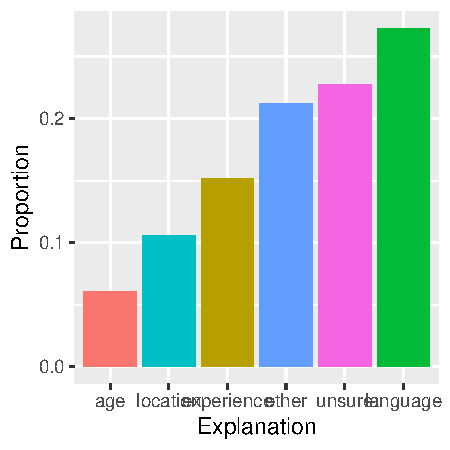
\includegraphics{figs/explanations-1} \caption[Children's explanations for why they think the target child knew or didn't know an animal]{Children's explanations for why they think the target child knew or didn't know an animal. Categories are not mutually exclusive.}\label{fig:explanations}
\end{figure}
\end{CodeChunk}

Of the 6 types of explanations, \emph{Language} was used by the highest
proportion of children (27.27\%). \emph{Unsure} and \emph{Other}
explanations contributed to just under half of all the explanations
(22.73\% and 21.21\% respectively). Of the remaining three types,
children appealed to \emph{Experience} the most (15.15\%), followed by
\emph{Location} (10.61\%) and \emph{Age} (6.06\%; see Figure
\ref{fig:explanations}). Note that because coding categories were not
mutually exclusive, the proportions sum to greater than 1. To understand
how children's explanations may change over development, we looked at
explanations in each age group. Perhaps unsurprisingly, \emph{Unsure}
explanations were more common in younger children, accounting for over
half (58.33\%) of the 4-year-olds' explanations.

Almost half of the 7- and 8-year-olds appealed to \emph{Language}
explanations (41.67\% and 45.45\%). Surprisingly, 5-year-olds were also
likely to use \emph{Language} explanations (38.46\%), while this type of
explanation was rarely used by 4- and 6-year-olds.

{[}\textbf{add elaboration about what we make of the pattern of
explanations, here or in discussion}{]}

\hypertarget{discussion}{%
\section{Discussion}\label{discussion}}

Our ability to infer other people's knowledge is crucial for successful
communication. Young children are capable of inferring others' general
knowledge states, but do they make accurate judgments about another
person's specific knowledge? We asked 4- to 8-year-old children to
estimate another child's knowledge of animal words, and found that
children as young as 4 are sensitive to a younger child's lexical
knowledge. Children across age groups made judgments similar to those of
adults, with older children recovering more adult-like patterns.

Our findings indicate that young children have surprising metalinguistic
knowledge, and can use that knowledge to make highly-specific inferences
about other people's knowledge. The animal words used in our study are
generally learned within a 6-month period, yet young children could
still distinguish early-acquired words from late-acquired words in this
set. Our study also builds upon the extant literature on children's
inferences about other people's knowledge to show that children infer
others' specific, lexical knowledge. When given fairly minimal
information about another child, children readily make estimates about
that child's lexical knowledge.

How are children in our study making estimates about other people's
knowledge? Children's own explanations suggest that they use various
cues to make their estimates. Language-related explanations were used by
the highest proportion of children, suggesting that even young children
rely on metalinguistic knowledge to make inferences about others.
{[}\textbf{adult work?}{]}. One limitation of the current study is that
it leaves the mechanisms underlying such estimates unclear. Future work
should could more directly probe the features underlying this
inference-- to see if children are relying on their own uncertainty,
word length (and other linguistic cues), features of the referent
itself, or still other features.

The current work lays the foundation for future research on how children
leverage their knowledge of other people to communicate successfully.
Young children struggle in a variety of communicative tasks (e.g. Krauss
\& Glucksberg, 1977), and the current work can begin to map out whether
such difficulties stem from tracking an interlocutor's knowledge, or may
stem from problems using that information to adjust language production.
By at least age 5, children selectively talk about general or specific
characteristics of an object based on their partners' knowledge state,
when the knowledge state is salient and explicit for each item (Baer \&
Friedman, 2018). Based on our findings that children can reason about
others' specific knowledge, we can ask whether children's adaptations
extend to the level of lexical knowledge-- Do children adjust the way
they talk about a referent based on their beliefs about a partners'
knowledge of that word?

\vspace{1em} \fbox{\parbox[b][][c]{7.3cm}{\centering Stimuli, data, and analysis code available after deanonymization.}}

\hypertarget{references}{%
\section{References}\label{references}}

\setlength{\parindent}{-0.1in} 
\setlength{\leftskip}{0.125in}

\noindent

\hypertarget{refs}{}
\begin{CSLReferences}{1}{0}
\leavevmode\hypertarget{ref-baer2018}{}%
Baer, C., \& Friedman, O. (2018). Fitting the message to the listener:
Children selectively mention general and specific facts. \emph{Child
Development}, \emph{89}(2), 461--475.

\leavevmode\hypertarget{ref-bates2015}{}%
Bates, D., Mächler, M., Bolker, B., \& Walker, S. (2015). Fitting linear
mixed-effects models using {lme4}. \emph{Journal of Statistical
Software}, \emph{67}(1), 1--48.
http://doi.org/\href{https://doi.org/10.18637/jss.v067.i01}{10.18637/jss.v067.i01}

\leavevmode\hypertarget{ref-birch2003}{}%
Birch, S. A., \& Bloom, P. (2003). Children are cursed: An asymmetric
bias in mental-state attribution. \emph{Psychological Science},
\emph{14}(3), 283--286.

\leavevmode\hypertarget{ref-cycowicz1997}{}%
Cycowicz, Y. M., Friedman, D., Rothstein, M., \& Snodgrass, J. G.
(1997). Picture naming by young children: Norms for name agreement,
familiarity, and visual complexity. \emph{Journal of Experimental Child
Psychology}, \emph{65}(2), 171--237.

\leavevmode\hypertarget{ref-fitneva2010}{}%
Fitneva, S. A. (2010). Children's representation of child and adult
knowledge. \emph{Journal of Cognition and Development}, \emph{11}(4),
458--484.

\leavevmode\hypertarget{ref-frank2017}{}%
Frank, M. C., Braginsky, M., Yurovsky, D., \& Marchman, V. A. (2017).
Wordbank: An open repository for developmental vocabulary data.
\emph{Journal of Child Language}, \emph{44}(3), 677--694.

\leavevmode\hypertarget{ref-galati2010}{}%
Galati, A., \& Brennan, S. E. (2010). Attenuating information in spoken
communication: For the speaker, or for the addressee? \emph{Journal of
Memory and Language}, \emph{62}(1), 35--51.

\leavevmode\hypertarget{ref-ghrear2020}{}%
Ghrear, S., Fung, K., Haddock, T., \& Birch, S. A. (2020). Only familiar
information is a {``curse''}: Children's ability to predict what their
peers know. \emph{Child Development}.

\leavevmode\hypertarget{ref-gopnik1988}{}%
Gopnik, A., \& Astington, J. W. (1988). Children's understanding of
representational change and its relation to the understanding of false
belief and the appearance-reality distinction. \emph{Child Development},
26--37.

\leavevmode\hypertarget{ref-jaswal2006}{}%
Jaswal, V. K., \& Neely, L. A. (2006). Adults don't always know best:
Preschoolers use past reliability over age when learning new words.
\emph{Psychological Science}.

\leavevmode\hypertarget{ref-krauss1977}{}%
Krauss, R. M., \& Glucksberg, S. (1977). Social and nonsocial speech.
\emph{Scientific American}, \emph{236}(2), 100--105.

\leavevmode\hypertarget{ref-kuperman2012}{}%
Kuperman, V., Stadthagen-Gonzalez, H., \& Brysbaert, M. (2012).
Age-of-acquisition ratings for 30,000 english words. \emph{Behavior
Research Methods}, \emph{44}(4), 978--990.

\leavevmode\hypertarget{ref-leung2021}{}%
Leung, A., Tunkel, A., \& Yurovsky, D. (in press). Parents fine-tune
their speech to children's vocabulary knowledge. \emph{Psychological
Science}.

\leavevmode\hypertarget{ref-lutz2002}{}%
Lutz, D. J., \& Keil, F. C. (2002). Early understanding of the division
of cognitive labor. \emph{Child Development}, \emph{73}(4), 1073--1084.

\leavevmode\hypertarget{ref-rossion2004}{}%
Rossion, B., \& Pourtois, G. (2004). {Revisiting Snodgrass and
Vanderwart's object pictorial set: The role of surface detail in
basic-level object recognition}. \emph{Perception}, \emph{33}, 217--236.

\leavevmode\hypertarget{ref-snodgrass1980}{}%
Snodgrass, J. G., \& Vanderwart, M. (1980). A standardized set of 260
pictures: Norms for name agreement, image agreement, familiarity, and
visual complexity. \emph{Journal of Experimental Psychology: Human
Learning and Memory}, \emph{6}(2), 174.

\leavevmode\hypertarget{ref-taylor1991}{}%
Taylor, M., Cartwright, B. S., \& Bowden, T. (1991). Perspective taking
and theory of mind: Do children predict interpretive diversity as a
function of differences in observers' knowledge? \emph{Child
Development}, \emph{62}(6), 1334--1351.

\leavevmode\hypertarget{ref-taylor1994}{}%
Taylor, M., Esbensen, B. M., \& Bennett, R. T. (1994). Children's
understanding of knowledge acquisition: The tendency for children to
report that they have always known what they have just learned.
\emph{Child Development}, \emph{65}(6), 1581--1604.

\leavevmode\hypertarget{ref-vanderborght2009}{}%
VanderBorght, M., \& Jaswal, V. K. (2009). Who knows best? Preschoolers
sometimes prefer child informants over adult informants. \emph{Infant
and Child Development: An International Journal of Research and
Practice}, \emph{18}(1), 61--71.

\leavevmode\hypertarget{ref-walley1992}{}%
Walley, A. C., \& Metsala, J. L. (1992). Young children's
age-of-acquisition estimates for spoken words. \emph{Memory \&
Cognition}, \emph{20}(2), 171--182.

\end{CSLReferences}

\bibliographystyle{apacite}


\end{document}
